\begin{figure}[H]
\centering

\begin{subfigure}{.16\textwidth}
  \centering
  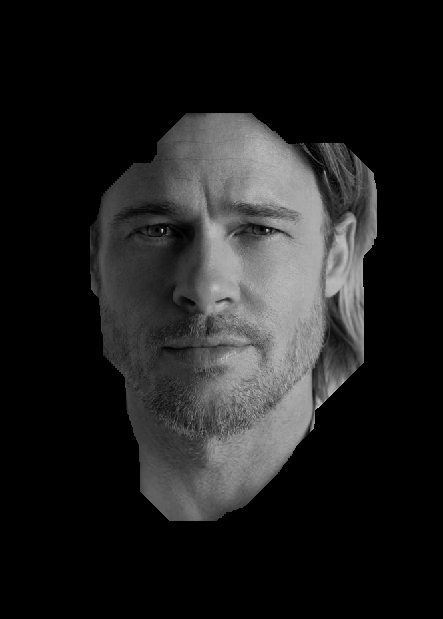
\includegraphics[width=0.95\textwidth]{img/fd3/grayFaceNormall.png}
  \caption{}
\end{subfigure}%
\begin{subfigure}{.16\textwidth}
  \centering
  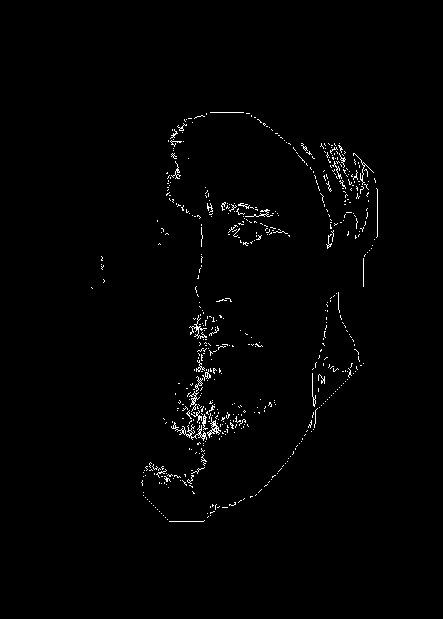
\includegraphics[width=0.95\textwidth]{img/fd3/grayFaceNormalFilteredFaceMask.png}
  \caption{}
\end{subfigure}%
\begin{subfigure}{.16\textwidth}
  \centering
  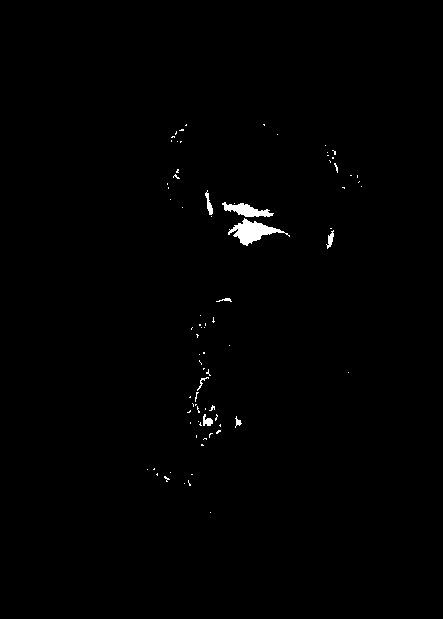
\includegraphics[width=0.95\textwidth]{img/fd3/grayFaceNormalEyeCandidates.png}
  \caption{}
\end{subfigure}%
\begin{subfigure}{.16\textwidth}
  \centering
  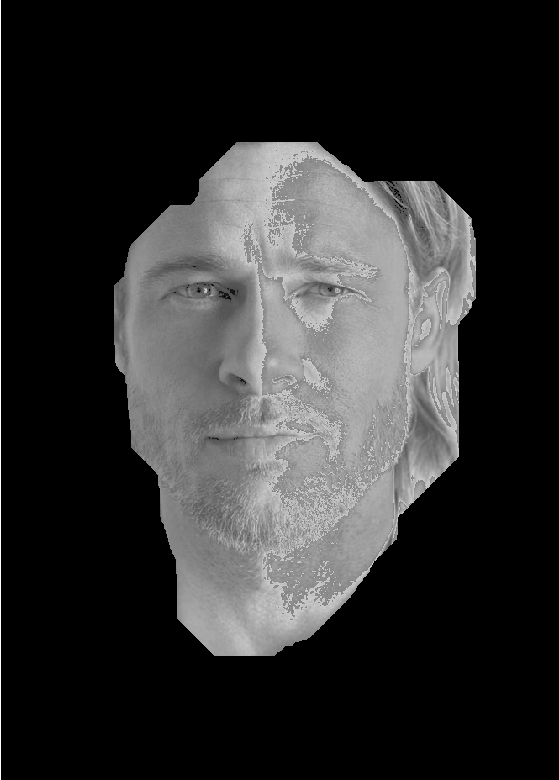
\includegraphics[width=0.95\textwidth]{img/fd3/grayFaceSpecial.png}
  \caption{}
\end{subfigure}%
\begin{subfigure}{.16\textwidth}
  \centering
  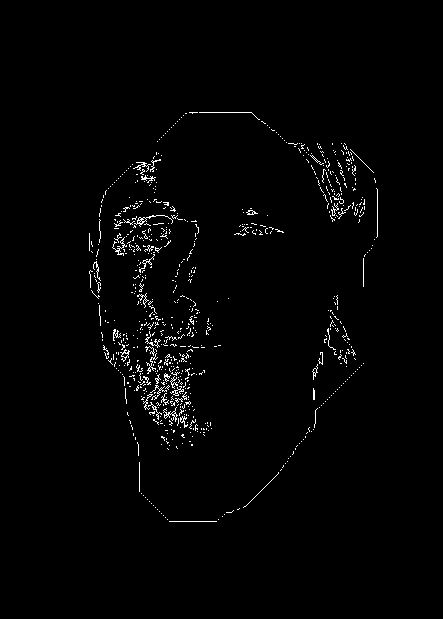
\includegraphics[width=0.95\textwidth]{img/fd3/grayFaceSpecialFilteredFaceMask.png}
  \caption{}
\end{subfigure}%
\begin{subfigure}{.16\textwidth}
  \centering
  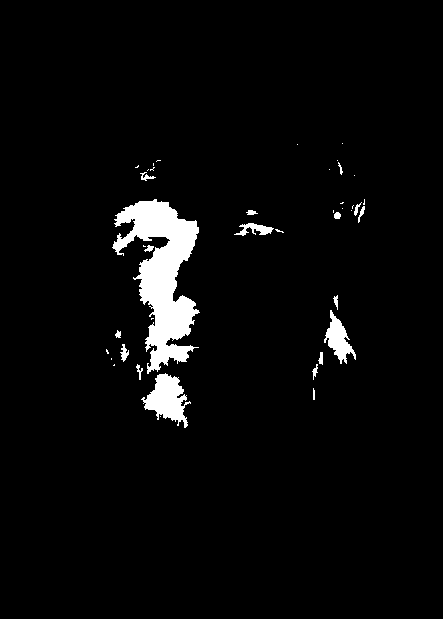
\includegraphics[width=0.95\textwidth]{img/fd3/grayFaceSpecialEyeCandidates.png}
  \caption{}
\end{subfigure}%

\caption{Process of equalizing the dark and bright part of a face being lit from the side. (a) show the original gray face image while (b) show filtered face mask and (c) the resulting eye candidates for the same image. (d) display the improved gray face image while (e) display the filtered face mask and (f) the eye candidates of this improved image.}
\label{fig:grayFace}
\end{figure}